\documentclass[12pt]{article}
\usepackage[utf8]{inputenc}
\usepackage{booktabs}
\usepackage{geometry}
\usepackage{graphicx}
\geometry{a4paper, margin=1in}
\title{Results of the Fisher Combined Test}
\author{Sara Fraija}
\date{\today}
\begin{document}
\maketitle
\section{Resultados}

\begin{table}[h!]
\centering
\resizebox{\textwidth}{!}{%
\begin{tabular}{l c c c c c c}
\toprule
\textbf{GRB} & \textbf{Transit} & \textbf{Significance} & \textbf{Significance Corregida} & \textbf{p-value} & \textbf{Corrected p-value} & \textbf{PDF} \\ \midrule
GRB170403583 & 1 & 1.01 & 0.82 & 8.438e-01 & 2.065e-01 & 7.604e-01 \\
GRB170826369 & 1 & 2.02 & 1.71 & 9.783e-01 & 4.366e-02 & 9.481e-01 \\
GRB190515190 & 1 & 0.00 & -0.82 & 5.000e-01 & 7.948e-01 & 6.011e-01 \\
GRB150101641 & 1 & 1.54 & 1.54 & 9.382e-01 & 6.178e-02 & 8.781e-01 \\
GRB150110923 & 1 & 2.08 & 2.08 & 9.812e-01 & 1.876e-02 & 9.541e-01 \\
GRB151229285 & 1 & 1.39 & 1.39 & 9.177e-01 & 8.226e-02 & 8.482e-01 \\
GRB160612842 & 1 & 0.00 & -0.00 & 5.000e-01 & 5.000e-01 & 6.011e-01 \\
GRB160624477 & 1 & 1.22 & 1.22 & 8.888e-01 & 1.112e-01 & 8.105e-01 \\
GRB160821937 & 1 & 2.28 & 2.28 & 9.887e-01 & 1.130e-02 & 9.703e-01 \\
GRB170318644 & 1 & 1.92 & 1.92 & 9.726e-01 & 2.743e-02 & 9.368e-01 \\
GRB170708046 & 1 & 2.02 & 2.02 & 9.783e-01 & 2.169e-02 & 9.481e-01 \\
GRB170803729 & 1 & 0.45 & 0.45 & 6.736e-01 & 3.264e-01 & 6.395e-01 \\
GRB170816599 & 1 & 2.13 & 2.13 & 9.834e-01 & 1.659e-02 & 9.587e-01 \\
GRB170817529 & 1 & 2.54 & 2.54 & 9.945e-01 & 5.543e-03 & 9.842e-01 \\
GRB180204109 & 1 & 1.93 & 1.93 & 9.732e-01 & 2.680e-02 & 9.380e-01 \\
GRB180418281 & 1 & 2.65 & 2.65 & 9.960e-01 & 4.025e-03 & 9.881e-01 \\
GRB180715755 & 1 & 0.96 & 0.96 & 8.315e-01 & 1.685e-01 & 7.484e-01 \\
GRB180718082 & 1 & 1.63 & 1.63 & 9.484e-01 & 5.155e-02 & 8.943e-01 \\
GRB180805543 & 1 & 0.99 & 0.99 & 8.389e-01 & 1.611e-01 & 7.556e-01 \\
GRB181125371 & 1 & 1.46 & 1.46 & 9.279e-01 & 7.215e-02 & 8.626e-01 \\
GRB190427190 & 1 & 2.59 & 2.59 & 9.952e-01 & 4.799e-03 & 9.861e-01 \\
GRB201008443 & 1 & 2.27 & 2.27 & 9.884e-01 & 1.160e-02 & 9.697e-01 \\
GRB201214672 & 1 & 2.85 & 2.85 & 9.978e-01 & 2.186e-03 & 9.931e-01 \\
GRB210323918 & 1 & 2.21 & 2.21 & 9.864e-01 & 1.355e-02 & 9.653e-01 \\
GRB210827416 & 1 & 0.59 & 0.59 & 7.224e-01 & 2.776e-01 & 6.648e-01 \\
GRB211024065 & 1 & 1.78 & 1.78 & 9.625e-01 & 3.754e-02 & 9.182e-01 \\
GRB220412713 & 1 & 2.34 & 2.34 & 9.904e-01 & 9.642e-03 & 9.742e-01 \\
GRB220418720 & 1 & 0.89 & 0.89 & 8.133e-01 & 1.867e-01 & 7.315e-01 \\
GRB220511571 & 1 & 2.49 & 2.49 & 9.936e-01 & 6.387e-03 & 9.820e-01 \\
GRB220617772 & 1 & 2.08 & 2.08 & 9.812e-01 & 1.876e-02 & 9.541e-01 \\
GRB221120895 & 1 & 1.26 & 1.26 & 8.962e-01 & 1.038e-01 & 8.196e-01 \\
GRB230228244 & 1 & 0.87 & 0.87 & 8.078e-01 & 1.922e-01 & 7.268e-01 \\
GRB230512269 & 1 & 1.95 & 1.95 & 9.744e-01 & 2.559e-02 & 9.404e-01 \\
GRB230812790 & 1 & 0.45 & 0.45 & 6.736e-01 & 3.264e-01 & 6.395e-01 \\
GRB170206453 & 2 & 0.10 & -0.55 & 5.398e-01 & 7.098e-01 & 6.030e-01 \\
GRB170403583 & 2 & 2.70 & 2.60 & 9.965e-01 & 4.716e-03 & 9.896e-01 \\
GRB170826369 & 2 & 3.03 & 2.81 & 9.988e-01 & 2.487e-03 & 9.960e-01 \\
GRB190515190 & 2 & 2.27 & 1.94 & 9.884e-01 & 2.632e-02 & 9.697e-01 \\
GRB150101641 & 2 & 0.75 & 0.75 & 7.734e-01 & 2.266e-01 & 6.989e-01 \\
GRB150110923 & 2 & 2.10 & 2.10 & 9.821e-01 & 1.786e-02 & 9.560e-01 \\
GRB151229285 & 2 & 1.01 & 1.01 & 8.438e-01 & 1.562e-01 & 7.604e-01 \\
GRB160624477 & 2 & 2.09 & 2.09 & 9.817e-01 & 1.831e-02 & 9.551e-01 \\
GRB160714097 & 2 & 0.00 & -0.00 & 5.000e-01 & 5.000e-01 & 6.011e-01 \\
GRB170318644 & 2 & 2.24 & 2.24 & 9.875e-01 & 1.255e-02 & 9.675e-01 \\
GRB170708046 & 2 & 2.14 & 2.14 & 9.838e-01 & 1.618e-02 & 9.596e-01 \\
GRB170803729 & 2 & 2.44 & 2.44 & 9.927e-01 & 7.344e-03 & 9.797e-01 \\
GRB170816599 & 2 & 1.92 & 1.92 & 9.726e-01 & 2.743e-02 & 9.368e-01 \\
GRB170817529 & 2 & 1.59 & 1.59 & 9.441e-01 & 5.592e-02 & 8.873e-01 \\
GRB171007498 & 2 & 0.85 & 0.85 & 8.023e-01 & 1.977e-01 & 7.220e-01 \\
GRB180204109 & 2 & 1.43 & 1.43 & 9.236e-01 & 7.636e-02 & 8.565e-01 \\
GRB180402406 & 2 & 3.08 & 3.08 & 9.990e-01 & 1.035e-03 & 9.965e-01 \\
GRB180418281 & 2 & 2.20 & 2.20 & 9.861e-01 & 1.390e-02 & 9.645e-01 \\
GRB180715755 & 2 & 1.37 & 1.37 & 9.147e-01 & 8.534e-02 & 8.439e-01 \\
GRB180718082 & 2 & 2.76 & 2.76 & 9.971e-01 & 2.890e-03 & 9.912e-01 \\
GRB180805543 & 2 & 2.44 & 2.44 & 9.927e-01 & 7.344e-03 & 9.797e-01 \\
GRB181125371 & 2 & 2.94 & 2.94 & 9.984e-01 & 1.641e-03 & 9.947e-01 \\
GRB190427190 & 2 & 0.17 & 0.17 & 5.675e-01 & 4.325e-01 & 6.068e-01 \\
GRB200623138 & 2 & 1.22 & 1.22 & 8.888e-01 & 1.112e-01 & 8.105e-01 \\
GRB201008443 & 2 & 2.90 & 2.90 & 9.981e-01 & 1.866e-03 & 9.940e-01 \\
GRB201214672 & 2 & 2.11 & 2.11 & 9.826e-01 & 1.743e-02 & 9.569e-01 \\
GRB210323918 & 2 & 0.28 & 0.28 & 6.103e-01 & 3.897e-01 & 6.164e-01 \\
GRB210618072 & 2 & 1.20 & 1.20 & 8.849e-01 & 1.151e-01 & 8.058e-01 \\
GRB210827416 & 2 & 1.41 & 1.41 & 9.207e-01 & 7.927e-02 & 8.524e-01 \\
GRB220412713 & 2 & 1.29 & 1.29 & 9.015e-01 & 9.853e-02 & 8.264e-01 \\
GRB220418720 & 2 & 2.54 & 2.54 & 9.945e-01 & 5.543e-03 & 9.842e-01 \\
GRB220511571 & 2 & 2.50 & 2.50 & 9.938e-01 & 6.210e-03 & 9.825e-01 \\
GRB220617772 & 2 & 3.14 & 3.14 & 9.992e-01 & 8.447e-04 & 9.971e-01 \\
GRB221120895 & 2 & 0.90 & 0.90 & 8.159e-01 & 1.841e-01 & 7.339e-01 \\
GRB230228244 & 2 & 3.10 & 3.10 & 9.990e-01 & 9.676e-04 & 9.967e-01 \\
GRB230512269 & 2 & 1.60 & 1.60 & 9.452e-01 & 5.480e-02 & 8.891e-01 \\
GRB230812790 & 2 & 1.98 & 1.98 & 9.761e-01 & 2.385e-02 & 9.438e-01 \\
GRB200605762 & 2 & 1.01 & 1.01 & 8.438e-01 & 1.562e-01 & 7.604e-01 \\
GRB150819440 & 2 & 2.22 & 2.22 & 9.868e-01 & 1.321e-02 & 9.661e-01 \\
GRB160612842 & 2 & 0.01 & 0.01 & 5.040e-01 & 4.960e-01 & 6.011e-01 \\
\bottomrule
\end{tabular}%
}
\caption{Lista de GRBs with sus Transits, Significances, Significances Corregidas, p-values, p-values Corregidos y valores PDF.}
\end{table}

\begin{figure}[h!]
\centering
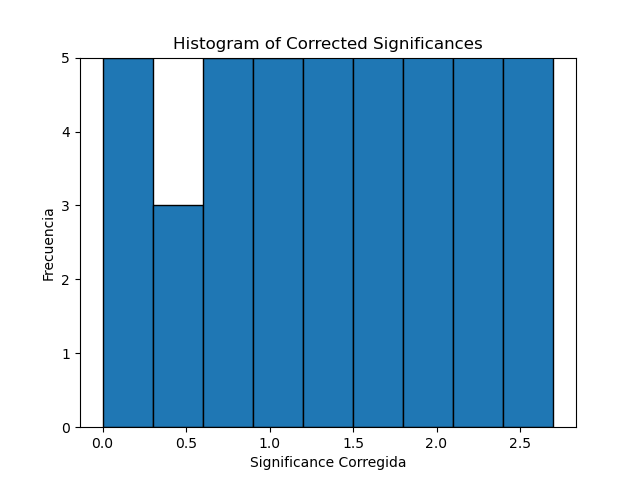
\includegraphics[width=0.6\textwidth]{corrected_significance_hist.png}
\caption{Histogram of Corrected Significances.}
\end{figure}

\section*{Conclusion}
The Fisher combined test integrates individual p-values to evaluate a global hypothesis.
The resulting test statistic was $X^2 = 499.364$ with 148 degrees of freedom.
For a significance level of 0.05, the critical value is 177.390.
Since $X^2$ is greater than the critical value, we rechazamos the null hypothesis of independence.
Normal approximation: p-value = 1.361e-38, significance ≈ 12.94 sigma.

\end{document}